%=====================================================================
\section{Proof of Minting}\label{sec:pom}

Minters collaborate to turn waiting payments into one minted block, certified by small zero-knowledge proofs, and share the block's fees by the work they did. The vocabulary is metalworking: a minter's address is its \emph{hammer}, a hash attempt is a \emph{blow}, a proving task is a \emph{strike}, the final proof is the \emph{stamp} and a full minted block is an \emph{ingot}.

\begin{figure}[tbp]
\centering
\begin{tikzpicture}[node distance=5mm and 11mm]
  \node[box,fill=copperwash,minimum width=2.4cm,minimum height=1.2cm] (blow) {\textbf{Blow}\\[-1pt]{\scriptsize Argon2id, 64 MB}\\[-2pt]{\scriptsize signed by the minter}};
  \node[box,right=of blow,minimum width=2.3cm,minimum height=1.2cm] (ticket) {\textbf{Ticket}\\[-1pt]{\scriptsize winning blow,}\\[-2pt]{\scriptsize 105 B in a block}};
  \node[box,right=of ticket,minimum width=2.4cm,minimum height=1.2cm] (cred) {\textbf{Credential}\\[-1pt]{\scriptsize ticket in the last}\\[-2pt]{\scriptsize $\approx$1,000 blocks (1.7 d)}};
  \node[box,right=of cred,minimum width=2.6cm,minimum height=1.2cm] (leaf) {\textbf{Leaf proof}\\[-1pt]{\scriptsize 4--16 payments}\\[-2pt]{\scriptsize Plonky2, 1.6--6.5 s}};
  \node[box,below=12mm of leaf,minimum width=2.6cm,minimum height=1.2cm] (tree) {\textbf{Hash tree}\\[-1pt]{\scriptsize of leaves, ranked}\\[-2pt]{\scriptsize by SHA256(minter, round)}};
  \node[box,left=of tree,minimum width=2.4cm,minimum height=1.2cm] (stamp) {\textbf{Stamp}\\[-1pt]{\scriptsize one Groth16 proof}\\[-2pt]{\scriptsize 196 B, 2--4 ms}};
  \node[box,left=of stamp,minimum width=2.3cm,minimum height=1.2cm,fill=bluewash] (seal) {\textbf{Seal}\\[-1pt]{\scriptsize miner, SHA-256}\\[-2pt]{\scriptsize 80-byte header}};
  \node[box,left=of seal,minimum width=2.4cm,minimum height=1.2cm] (block) {\textbf{Block}\\[-1pt]{\scriptsize fees: 75\% provers,}\\[-2pt]{\scriptsize 25\% miner}};
  \draw[arr] (blow) -- node[lbl,above=2pt] {wins} (ticket);
  \draw[arr] (ticket) -- (cred);
  \draw[arr] (cred) -- node[lbl,above=2pt] {claims} (leaf);
  \draw[arr] (leaf) -- (tree);
  \draw[arr] (tree) -- (stamp);
  \draw[arr] (stamp) -- (seal);
  \draw[arr] (seal) -- (block);
\end{tikzpicture}
\caption{Minting a block. Blows win tickets; a ticket in the recent chain is a credential; credentialed minters prove leaves of payments; leaves are merged into one stamp, and the miner seals the block.}
\label{fig:pipeline}
\end{figure}

\subsection{Blows}
A blow is one attempt at a memory-hard puzzle, signed with the minter's own account key, the key that also signs its payments \st{Decided; one key per person, Decided October 2026}:
\begin{align*}
m &= \mathrm{Poseidon}(\text{``ZenBlow''},\ \text{chain},\ \text{block}_{k-1},\ \text{nonce})\\
(e, s) &= \mathrm{Schnorr}_{\text{EcGFp5}}(\text{account key},\ m) \qquad \text{(deterministic)}\\
\mathit{blow} &= \mathrm{Argon2id}\big(\text{block}_{k-1}\,\|\,A\,\|\,\text{nonce}\,\|\,e\,\|\,s;\ \text{salt ``Zen-blow-v1''};\ 64\,\text{MB},\ 1\text{ pass},\ 1\text{ lane}\big)
\end{align*}
A blow wins when it is below the blow target. Everyone checks a winning blow with one signature check and one Argon2id run, with no state: the 105-byte ticket carries the compressed public key $A$ (41 bytes), the nonce, $e$ and $s$. The signature means only the key holder can make attempts for that key, and nobody can claim another minter's blow. Because the minting key is the account key, the ticket, the credential, the minters' coins and the leaf fees all reach one address, and handing the key to a pool would hand over the account's money: minting stays personal. Payment messages begin with the chain id and blow messages with the tag, so one signature never passes as the other, and a blow counts on one chain only. A minter may sign the same nonce twice, but each signature costs its own Argon2id run; a block counts one ticket per address and nonce. In Rust, on one server core, signing takes 1.2\,ms and an attempt 84\,ms; a node checks a ticket in about 75\,ms (measured). The 64\,MB of memory, refilled for every attempt, keeps dedicated chips from gaining a large advantage over phones and computers.

\begin{figure}[htbp]
\centering
\begin{minipage}[t]{0.48\textwidth}\centering
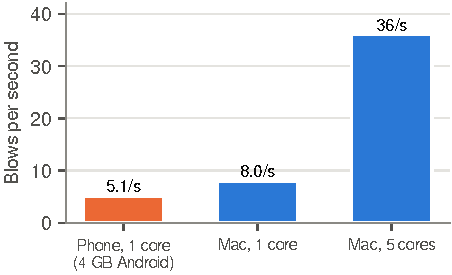
\includegraphics[width=\textwidth]{figs/blowbench.pdf}
\caption{Blows per second in a browser (Jen Minting Bench, 10 October 2026, measured). A phone takes 191--201\,ms per blow; a 10-core Mac 125\,ms per core. Neither slowed from heat over 4 minutes.}
\label{fig:blowbench}
\end{minipage}\hfill
\begin{minipage}[t]{0.48\textwidth}\centering
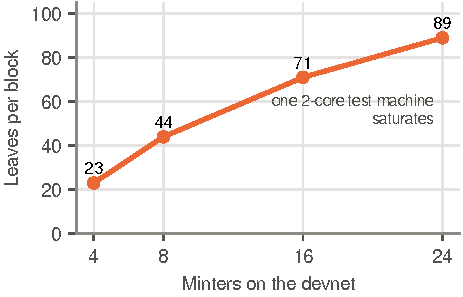
\includegraphics[width=\textwidth]{figs/capacity.pdf}
\caption{Collaborative minting on the Jen-0.8 devnet: leaves per block as minters are added (proving simulated at 2\,s per leaf). Capacity grows with minters until the single test machine saturates.}
\label{fig:capacity}
\end{minipage}
\end{figure}

The blow difficulty aims at a fixed number of winning blows per block, 24 on the real chains: after each block, $\text{new} = \text{old}\times(3\,\text{target} + \text{blows})/(4\,\text{target})$, limited to $\pm12.5\%$ per block \st{Decided}. More minters make blows harder, not blocks bigger. Checking 24 blows costs about 3\,s of one desktop core per 2.5-minute Jen block (measured).

\subsection{Tickets, credentials and the minting gate}
Every winning blow becomes a \emph{ticket}, a record of (public key, nonce, signature) of 105 bytes carried in the block \st{Decided, Jen-0.8; size from the Rust port}. Tickets do three things:
\begin{itemize}
\item \textbf{The minting gate.} A block is valid only with enough minting work: at least a third of the recent average minting work per block, counted as the sum of the blow difficulties, and never less than one blow at the current difficulty. A chain cannot meet the gate by lowering its own blow difficulty.
\item \textbf{New coins.} The minters' part of each block's new coins goes into a pool; each block's tickets share $1/32$ of the pool. On the devnet each minter's share of the minters' coins came within 2--4 points of its share of blows.
\item \textbf{Credentials.} A minter with a ticket in the chain within the last \textit{CredBlocks} blocks is credentialed: about 1,000 blocks, roughly 1.7 days, on the real chain. The ticket was verified when its block arrived, so checking a credential is a lookup.
\end{itemize}
In a three-minute quiet test with no payments sent, blocks kept coming every 16.7\,s with 51 tickets in 11 blocks (devnet): tickets keep the chain alive when nobody pays.

\subsection{Leaves: proving payments}
Any credentialed minter may claim waiting payments and prove \emph{leaves}, groups of 4 to 16 payments, one after another, as fast as its device allows \st{Decided, Jen-0.8}. Since October 2026 a leaf has two halves \st{Proposed, measured}:
\begin{itemize}
\item a \textbf{signature leaf}, proved by the minter, checks each payment's signature, the fee band and the floors in coins. It knows no balances and no tree, so any number of minters prove at the same time without knowing each other's leaves. Its public values are the hash of its signed payments with the minter's address, and $S$;
\item a \textbf{state leaf}, proved by the block builder, verifies one signature leaf inside it, repeats the signed fields (their hash must match, so the builder cannot change a payment, a nonce or the minter's address) and applies the payments to the account tree in order. A payment that no longer fits the state is \emph{skipped}: no change, no fee, absent from the block data.
\end{itemize}

\begin{table}[htbp]
\centering\small
\begin{tabular}{l r r r r}
\toprule
\textbf{Leaf size} & \textbf{Rows} & \textbf{Proving time} & \textbf{Memory} & \textbf{Proof}\\
\midrule
Signature leaf, 4 payments & $2^{12}$ & 1.4 s & 0.5 GB & 124 KB\\
Signature leaf, 16 payments & $2^{14}$ & 5--6 s & 0.9 GB & 143 KB\\
State leaf, 16 slots (builder) & $2^{13}$ & 2.7 s & 0.9 GB & 130 KB\\
\bottomrule
\end{tabular}
\caption{Leaf proofs, signatures checked inside the signature leaf: Plonky2 (FRI, no trusted setup, Poseidon over the Goldilocks field) on a 2-core server, October 2026 (measured; phones not yet tested). The Go prototype's Groth16 leaves (MiMC, gnark) took 3.8\,s for 4 payments and 13.9\,s for 16, with 164-byte proofs.}
\label{tab:leaf}
\end{table}

Leaves are ranked by $\mathrm{SHA256}(\text{minter identity}, \text{round}, \text{leaf})$. The rank fixes their order in the block and settles clashes. The block body is a hash tree of leaves and the miner seals its root. Each leaf's prover earns 75\% of that leaf's fees. With the stamp (Section~\ref{sec:stamp}) nodes check one proof per block instead of one per leaf; only blows cost an Argon2id check, so blows stay near 100 per block while leaves grow with the number of minters (Figure~\ref{fig:capacity}).

\paragraph{Fairness between fast and slow provers.} Two rules (Jen-0.10) keep one large prover, or a miner ordering its own leaves first, from filling a block: a \emph{leaf quota} (a minter may place at most $\tfrac54\times\text{cap}\times$ its share of tickets in the credential window, at least one leaf) and a \emph{split payment pool} (each payment falls in one bucket per round, $\mathrm{hash}(\text{payment},\text{round}) \bmod$ the number of credentialed minters, and each minter proves its own bucket first). On a six-node devnet with ten times more traffic than minters could prove, these rules cut wasted overlapping proofs from 78\% to 3\%, raised payments per block from 36 to 208, and cut the share of a prover 15 times faster than the rest from 99\% to 23\% of leaves (Figure~\ref{fig:ab}).

\begin{figure}[htbp]
\centering
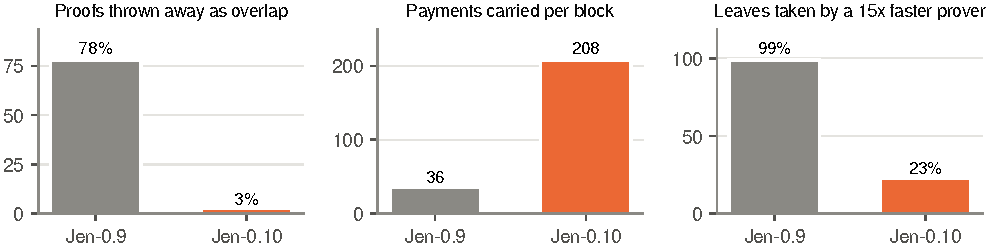
\includegraphics[width=\textwidth]{figs/ab.pdf}
\caption{Devnet A/B test, six nodes, traffic ten times what minters can prove: Jen-0.9 rules against Jen-0.10 (leaf quota and split pool). All nodes agreed and supply was exact in both (devnet).}
\label{fig:ab}
\end{figure}

\subsection{The same payment at two minters}
A payer can send two conflicting payments, with the same nonce, to two minters who prove them in parallel. Both proofs can be valid on their own; only one can be in the chain. Zen handles this in three layers:
\begin{enumerate}
\item The split pool sends all of a sender's payments in a round to the same bucket, so honest double proving is rare.
\item Within a block, leaves are applied in rank order. The builder's state leaf skips a payment whose (sender, nonce) is already used; only that payment is lost, and its minter earns no fee for it.
\item The clash is detected by (sender, nonce), not by payment ID, so two different payments with the same nonce always clash \st{Proposed for specification 4.10}.
\end{enumerate}
Signature leaves hold no state, so a conflicting payment costs its minter only that payment's fee, not the whole leaf. On a 128-slot block, a double spend (same sender, same nonce, two receivers) and a replayed payment were both skipped and the other payments applied (measured).

\subsection{Merging and the stamp}\label{sec:stamp}
In the Go prototype each node verifies every leaf proof (about 1\,ms each), which caps a block at 1,024 leaves, sized for a phone verifier \st{Decided, Jen-0.9}. A Rust benchmark written for this paper (October 2026) merges the leaves of a block into a single \emph{stamp} that any node checks in 2--4\,ms \st{Proposed, measured}. A block of 8 leaves of 16 payments goes through five stages (Figure~\ref{fig:zkpipeline}):
\begin{enumerate}
\item \textbf{Leaves} (Plonky2): signature leaves on minters' devices (16 payments, 5--6\,s), then state leaves on the builder (2.7\,s each), which apply the payments, move the state root and add the payouts (Section~\ref{sec:blockdata}).
\item \textbf{Merges} (Plonky2 recursion): a merge verifies two child proofs, checks that the left one's root after is the right one's root before, adds their fees and counts, and hashes their data commitments. Seven merges turn 8 leaves into one proof; each takes about 2.7\,s.
\item \textbf{Shrink} (Plonky2): the stamp is proved once more into a smaller circuit, $2^{13}$ rows.
\item \textbf{BN254 layer} (Plonky2): the same proof again, with its Merkle trees hashed by Poseidon over the BN254 field, so the next step can check it cheaply.
\item \textbf{Stamp} (Groth16 on BN254, gnark v0.16.4): a circuit of 4.2 million constraints verifies the whole BN254-layer proof and outputs 196 bytes. It needs 6\,GB and 96--112\,s on 2 cores; gnark's GPU prover (ICICLE) produces the same proof on an NVIDIA card.
\end{enumerate}

\begin{figure}[htbp]
\centering
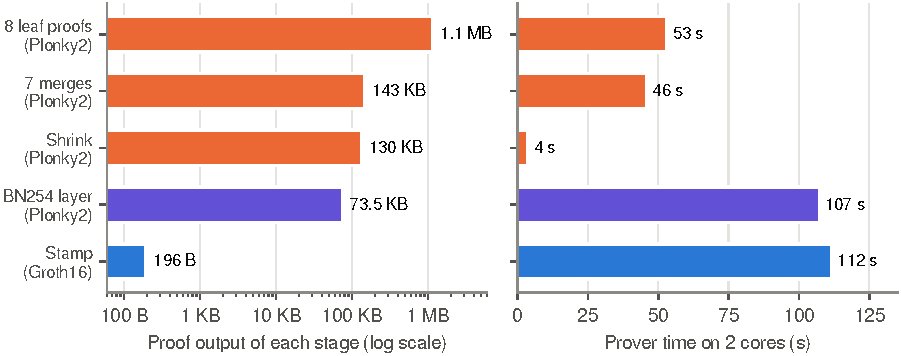
\includegraphics[width=\textwidth]{figs/zkpipeline.pdf}
\caption{A block of 128 signed payments from leaf proofs to one stamp: what each stage outputs (left, log scale) and the prover time it needs on a 2-core server (right). Orange: Plonky2 with Poseidon over Goldilocks; violet: Plonky2 with Poseidon over BN254; blue: Groth16. Leaves and merges run in parallel across minters; the times here are for one machine doing everything (measured, October 2026).}
\label{fig:zkpipeline}
\end{figure}

\paragraph{Why two proof systems.} Plonky2 proofs need no trusted setup and recurse cheaply, but each is 70--150\,KB. A Groth16 proof is 196 bytes and checks in milliseconds, but its key belongs to one circuit and needs a setup ceremony. Wrapping only the last step keeps the ceremony to one fixed circuit and keeps all the work that changes with traffic free of it. Without the wrap, the stamp is a 70\,KB Plonky2 proof with no setup at all, checked in about 3\,ms \st{Open: which one ships}. The Groth16 verifier is the open-source gnark verifier for Plonky2, ported to current Plonky2 and gnark; the port needed three changes, all from Plonky2 updates (the transcript now absorbs the FRI parameters, and two field generators changed).

\paragraph{Signatures inside the proof.} Proving is paid work and verification should stay cheap, so signatures are checked inside the leaf proofs and never published: a signature of 64 bytes or more per payment would be five times the 13-byte payment record. A custom gate computes $2P + Q$ on the curve in one operation, two per row, and one loop over the 319 bits of $s$ handles $s\cdot G$ and $e\cdot A$ together, which cut a 16-payment leaf from 30.7\,s and 4.3\,GB to about 5\,s and 0.6\,GB. The circuit checks that $s<n$, that the challenge is decoded canonically, that both points are on the curve, and that the addition formulas never meet an exceptional case. A forged signature produces no proof.

\paragraph{One key for every block size.} State-leaf proofs and merge proofs are built with exactly the same circuit shape: the same number of rows ($2^{13}$ since the leaf split), the same gate types and the same 84 public values. One \emph{universal merge} circuit can then verify either kind of child with a single verifier, switching only the key: the leaf's fixed key, or the merge circuit's own key, which every merge proof carries in its public values and must pass on to its parent. A lone child passes through. Any number of leaves therefore ends in a proof of the same circuit, and everything above it, including the Groth16 key, never changes. Blocks of 8, 3 and 1 leaves (128, 40 and 5 payments) produced identical final circuits and were proved and verified with one Groth16 key from one 20-minute setup; one block's proof checked against another block's public values was rejected. Merges got cheaper with the smaller shape, about 2.7\,s each. Within a leaf, unused slots are padding: they change no account, add no fee and are not counted.

\paragraph{Operations inside the stamp.} \st{Proposed, testnet} Payments are only part of a block. The chain also holds \emph{locks}, leaves of the account tree whose address is a digest of their terms: vaults, exchange orders and auctions, channels and channel factories (Sections~\ref{sec:channels} and~\ref{sec:exchange}). Each lock operation moves coins between an account and a lock, or between two states of one lock, so it changes the account tree like a payment does. Since the Rust test network reached this stage, four more leaf circuits sit beside the state leaf, one per family: \emph{vault} (make, claim, refund), \emph{channel} (make, fund, start, update, settle, close, streams, with up to eight point locks opened inside the circuit), \emph{order} (make, reserve, bid, reopen, return, claim) and \emph{factory} (up to eight members, make, fund, start, post, exit, exit now). Every leaf is built to the same shape as the state leaf ($2^{13}$ rows, the same gates, 84 public values), so the universal merge takes any mix of them: it now holds the verifier keys of the state leaf and the four operation leaves and picks one by a flag per child. A block with a payment, an order, a channel and a factory is one tree and one 196-byte stamp. Two format changes made this possible. Lock addresses and every signed message use Poseidon over field elements, not SHA-256, because one SHA-256 compression costs tens of thousands of gates; and the size of every list (point locks, factory members) has a fixed maximum. The block data hash commits to each operation in block order, as it does for payments.

The circuits check the rules a node checks (who may sign, the balances, the time windows, the update number, the shares, the opening of a point lock) with one deliberate exception: a few checks stay with the node, because they would cost many rows in the circuit. These are that a public key is in the right subgroup and matches its address, the sign of a curve point's $y$, that a new address is not already used, that the members of a factory are distinct, and the \emph{foreign payment proof} of an order claim. The last matters for the exchange: the circuit checks that the order is reserved, that the claim is inside the reservation, that the whole locked balance goes to the taker and that the sender signed the digest of the payment proof, but the other chain's header chain and block body are not in the circuit. Every node still checks that proof when it accepts the block. A stamp therefore tells a light client that the node rules were applied, and a full node re-checks the foreign payment; to make the stamp cover it would need the other chain's headers as public input and a block-body hash inside the circuit, a much larger step.

\paragraph{Testing the circuits against the node.} A circuit is sound if it cannot prove an operation that the node refuses. For each family a test walks a story of real operations and, at every step, tries to break it: one field changed (amount, fee, destination, sender, signature byte, terms, lock index, proof digest); the same operation tried six blocks before and after its true height, so that every time rule is tested on both sides of its edge; fee variants; and rule-breaking variants specific to the family (an unfunded make, an early reopen, a bid that does not beat the last, a claim after the window, an update number of zero, shares beyond the channel, a wrong point-lock scalar, an early exit, a forged member signature). A try passes if the circuit does not prove it, or proves exactly the honest operation. In all, 583 tries (vault 62, channel 181, order 196, factory 144) gave no failure. To check that the tests can see a bug, one rule (the order reopen window) was removed on purpose; eleven tries then failed, and the rule was restored (testnet). These tests are a probe and not a proof; they do not cover the node-only checks above, and they were run on a single-party setup (next paragraph).

\paragraph{The setup.} The Groth16 key of the operation-carrying circuit was made on one machine for the test network: 4.2 million constraints, a 2\,GB proving key, a 1,008-byte verifying key, about 17 minutes. Whoever runs such a setup could keep its secret randomness and forge stamps, so this key is for testing only. A launch needs a public multi-party ceremony for exactly this circuit \st{Open}; the 70\,KB Plonky2 stamp, which needs none, remains the fallback.

\paragraph{Who proves what, and when.} Every block carries its stamp \st{Decided, October 2026}. The protocol names no machine: a builder too slow to finish the stamp misses the block, and someone faster seals it. Minters prove signature leaves on phones and PCs; the builder, in practice a mining pool, proves state leaves, merges and the BN254 layer on server cores and the Groth16 stamp on an NVIDIA GPU through gnark's ICICLE backend, which reads the same proving key and produces the same 196-byte proof; miners seal with SHA-256 ASICs. On 2 cores the builder's work takes about 3.7 minutes; the target is about 60 seconds after the last leaf, inside Jen's 2.5-minute block. The GPU prover is built but not yet measured, so this target is open until a benchmark on a many-core GPU server. The peg's account fields (Section~\ref{sec:defences}) are in the account leaf and the state leaf (Rust, round 13), and none of the circuits is audited.

\subsection{Block data and node checks}\label{sec:blockdata}
A stamp proves that the new state root is right, but a root alone tells nobody their balance, and the next prover needs the whole tree. So every block publishes its payments (without signatures), and the stamp \emph{commits} to them: each leaf hashes its slot entries (unused flag, sender, receiver, amount, fee, new-account and close flags, a new account's address) and its prover's address, and each merge hashes the two child hashes. The stamp's 16 public values are the root before and after, the fee total, the payment count, this data hash, $S$ and the block height \st{Proposed, measured}. A node accepts a block when, in order:
\begin{enumerate}
\item its root before equals the previous block's root after;
\item the stamp verifies with the 16 public values;
\item the payment bytes decode cleanly (minimal integers, no trailing bytes);
\item replaying the payments on its own copy of the state, with the rules of Section~\ref{sec:accounts}, gives the same root after, fee total, count and data hash.
\end{enumerate}
A block of 128 payments measured 1,940 bytes: 1,632 of payments (12.6 bytes each), 13 of header and counts, 112 of public values and 196 of stamp, about 15 bytes per payment. With the version-2 leaf header (37 bytes per leaf: count, new-account and close masks, prover address) and 21 payments creating accounts, a block of 128 payments carried 2,596 bytes of data. Changing one byte of the payment data made the replay disagree. The signed message includes the sender's nonce and the proof increments it, so a payment re-submitted with its original signature is skipped and never applied twice.

\paragraph{Minters are paid by lottery.} The minters' share of a block goes straight to that block's 24 winning tickets, equal shares each, one credit per address; no node keeps a ledger of what minters are owed. The number of credits a block spends on minters is therefore at most 24, whether there are a hundred minters or a billion: more minters only raise the difficulty. In a simulation of 100 to 300,000 minters, a block carried 18 to 24 credits, and pay followed work (the top 1\% of minters earned 35.6\% of the pay for 35.2\% of the work). The price is variance: a small solo minter wins rarely, about once in (minters $/$ 24) blocks, so steady income comes from minting pools, which are ordinary addresses that split what they win with ordinary payments. An earlier design that paid every minter once every 32 blocks was dropped, because its saving fell to 1.6$\times$ at 10,000 minters \st{Decided}.

\paragraph{Payouts inside the proof.} A slot that a signature leaf left empty can carry a \emph{credit}: no sender, no signature, an amount added to an account, which is created on first receipt \st{Proposed, measured}. Every node computes the payouts a block owes: half of each leaf's fees goes into a fee pool, 75\% of the rest to the leaf's prover and the remainder to the miner; the pool pays 1/32 of what it held per block, 75\% to the block's provers and the rest to the miner; rewards owed from block $h-2$ come first (75/25 \st{Open}). A block is valid only if its credits, in order, are exactly that list, and the proof shows that each one reached the account tree. A leaf with no payments is credit-only and reuses one empty signature leaf. In a 128-slot block, 110 payments and 11 credits, one of them opening a minter's account, took 2,401 bytes (version 4: each leaf header carries payment, credit, new-account and close masks and the prover, 40 bytes). A builder that paid one unit too much produced a valid proof, and nodes rejected the block (measured).

\begin{figure}[tbp]
\centering
\begin{tikzpicture}[
  lf/.style={draw=jen,fill=copperwash,rounded corners=1.5pt,minimum width=1.25cm,minimum height=0.62cm,font=\sffamily\scriptsize,align=center,line width=0.6pt},
  hn/.style={draw=ink2,fill=white,rounded corners=1.5pt,minimum width=1.2cm,minimum height=0.5cm,font=\sffamily\scriptsize,line width=0.6pt}]
  % header
  \node[box,fill=bluewash,minimum width=13.6cm,align=left,anchor=west] (hdr) at (0,4.3) {\textbf{Seal (80 bytes, Bitcoin layout):} version \textbar{} previous block \textbar{} commitment \textbar{} time \textbar{} bits \textbar{} nonce};
  \node[box,minimum width=13.6cm,align=left,anchor=west] (com) at (0,3.35) {\textbf{Commitment} = SHA256d(SHA256d(coinbase) \textbar{} body root); coinbase: chain, height, extra nonces, miner};
  % tickets
  \node[box,fill=wash,minimum width=4.2cm,minimum height=2.3cm,anchor=north west,align=left] (tk) at (0,2.75) {\textbf{Tickets}\\[1pt]{\scriptsize $\approx$24 winning blows}\\[-1pt]{\scriptsize (public key, nonce, signature)}\\[-1pt]{\scriptsize 105 B each, $\approx$2.5 KB}\\[-1pt]{\scriptsize gate, new coins, credentials}};
  % tree
  \node[hn] (r) at (9.3,2.35) {leaf root};
  \node[hn] (a) at (7.2,1.45) {hash};
  \node[hn] (b) at (11.4,1.45) {hash};
  \node[lf] (l1) at (5.8,0.35) {leaf 1\\4--16 pay};
  \node[lf] (l2) at (7.3,0.35) {leaf 2};
  \node[lf] (l3) at (8.8,0.35) {leaf 3};
  \node[lf] (l4) at (10.3,0.35) {leaf 4};
  \node[font=\sffamily\small] at (11.55,0.35) {$\cdots$};
  \node[lf] (l5) at (12.8,0.35) {leaf $n$};
  \draw[line width=0.6pt,color=ink2] (r) -- (a); \draw[line width=0.6pt,color=ink2] (r) -- (b);
  \draw[line width=0.6pt,color=ink2] (a) -- (l1); \draw[line width=0.6pt,color=ink2] (a) -- (l2);
  \draw[line width=0.6pt,color=ink2] (b) -- (l3); \draw[line width=0.6pt,color=ink2] (b) -- (l4); \draw[line width=0.6pt,color=ink2] (b) -- (l5);
  \node[lbl,anchor=north] at (9.3,-0.15) {each leaf: payments ($\approx$13 B each) + prover; ordered by rank; merged into one stamp};
  \draw[arr,dashed] (r.north) -- (9.3,3.05);
  \node[box,minimum width=2.6cm,anchor=west,align=left] at (11.0,2.35) {\textbf{Stamp:} \scriptsize 196 B\\[-1pt]\scriptsize + 16 public values};
\end{tikzpicture}
\caption{Structure of a minted block. The miner's 80-byte seal commits to everything else, so miners cannot change a minted block. For example, 24 tickets (2.5\,KB), 660 payments (about 8.6\,KB at 13\,B each) and one stamp with its public values (324\,B) make a block of about 11.5\,KB (estimate).}
\label{fig:block}
\end{figure}

%=====================================================================
\section{Mining and consensus}\label{sec:mining}

\subsection{The seal}
Miners seal each minted block with double SHA-256 over Bitcoin's exact 80-byte header: version, previous block, a commitment, time, compact difficulty bits and a 32-bit nonce, in Bitcoin's byte order \st{Decided, Jen-0.5; Bitcoin-exact since October 2026}. The commitment is built as a Bitcoin merkle root over a one-transaction coinbase and one branch, $\mathrm{SHA256d}(\mathrm{SHA256d}(\text{coinbase})\,\|\,\text{body root})$: the coinbase holds the chain, the height, the pool's and miner's extra nonces and the miner's address, and the body root hashes everything minted (Figure~\ref{fig:block}), so a miner cannot alter a minted block. This is exactly what Stratum v1 pools and their miners compute, so existing SHA-256 chips, firmware and pools seal Zen blocks unchanged, version rolling included; a pool puts its own address in the coinbase and pays its miners as it does for Bitcoin. No private key is needed and pools are allowed. Our header code reproduces Bitcoin's genesis block hash; a miner that knew only Stratum found a seal the node accepted, and a seal reused for a changed block, a swapped miner address and a seal shown to another chain were rejected (measured). Mining and minting are deliberately different: minting is personal, memory-hard and phone-friendly; sealing is anonymous, poolable and uses the world's largest installed hashing base.

\subsection{Two-factor fork choice}
The chain with the most total weight wins; at equal height the lower seal hash wins \st{Decided, Jen-0.5}. Each block's weight counts both kinds of work:
\begin{equation}
\mathrm{Weight}(B) = D_{\mathrm{seal}}\cdot\frac{\min(\mathrm{blows}_B,\ 2\bar b)}{\bar b},\qquad \bar b \leftarrow \bar b + \frac{\mathrm{blows}_B - \bar b}{32}.
\end{equation}
A chain sealed with much hashing but little minting weighs little. In hidden-chain attacks on the Jen-0.5 devnet, an attacker with three times the honest sealing power built in secret for four minutes and then published. With seal work alone, an attacker with half the honest minting made honest nodes abandon 17 blocks; with two-factor weight the same attacker reached only 59\% of the honest weight and failed, though its chain was three blocks longer (Figure~\ref{fig:hidden}).

\begin{figure}[htbp]
\centering
\begin{minipage}[t]{0.48\textwidth}\centering
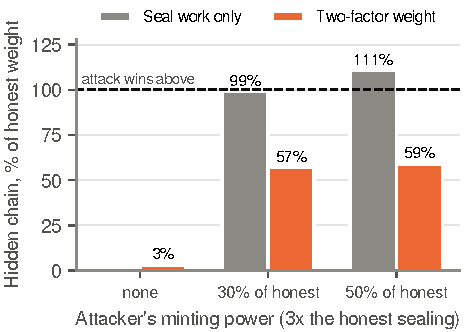
\includegraphics[width=\textwidth]{figs/hidden.pdf}
\caption{Hidden-chain attacks on the Jen-0.5 devnet with three times the honest sealing power. Bars show the hidden chain's weight as a share of the honest chain's (devnet).}
\label{fig:hidden}
\end{minipage}\hfill
\begin{minipage}[t]{0.48\textwidth}\centering
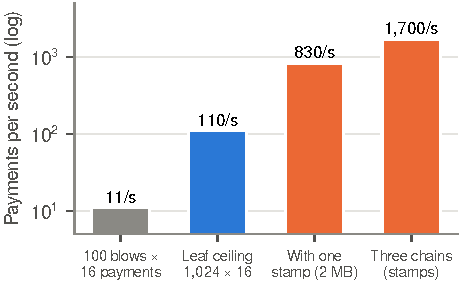
\includegraphics[width=\textwidth]{figs/throughput.pdf}
\caption{Jen throughput levers (estimates). Today, 24 blows each carrying up to 16 payments; then the 1,024-leaf ceiling; then one stamp per block, filling the 2\,MB ceiling; then all three chains.}
\label{fig:throughput}
\end{minipage}
\end{figure}

\subsection{Difficulty and launch}
Two difficulties run side by side: the blow difficulty keeps winning blows near their target per block (Section~\ref{sec:pom}), and the seal difficulty keeps each chain at its block time \st{TBD numbers}. A retarget that only acts when a block arrives has a weakness at launch and when miners leave suddenly: if the difficulty is set for far more hashing than is present, the next block is slow, and each slow block only lowers the difficulty one step. Zen therefore proposes a \emph{time-based} difficulty (in the style of ASERT): the target a block must meet is computed from how far the chain is ahead of or behind its schedule, so the difficulty keeps falling while nobody finds a block \st{Proposed}:
\begin{equation}
D(t) = D_{\mathrm{ref}}\cdot 2^{\,(N T - t)/h},
\end{equation}
where $N$ is the number of blocks since the reference block, $T$ the block time, $t$ the time since the reference block and $h$ the half-life. Figure~\ref{fig:launch} compares the two rules on Jen in a simple simulation made for this paper. With a genesis difficulty set for fifty times the hashing that shows up, per-block retargeting needs about 28 hours to reach block 100 instead of about 4; the time-based rule with a one-hour half-life needs about 10. When 90\% of the hashing leaves suddenly, per-block retargeting takes about 10.6 hours to reach block 100 against 4.4 for the time-based rule. The same rule applies to the blow target, so a minting gate never blocks a young chain with few minters.

\begin{figure}[htbp]
\centering
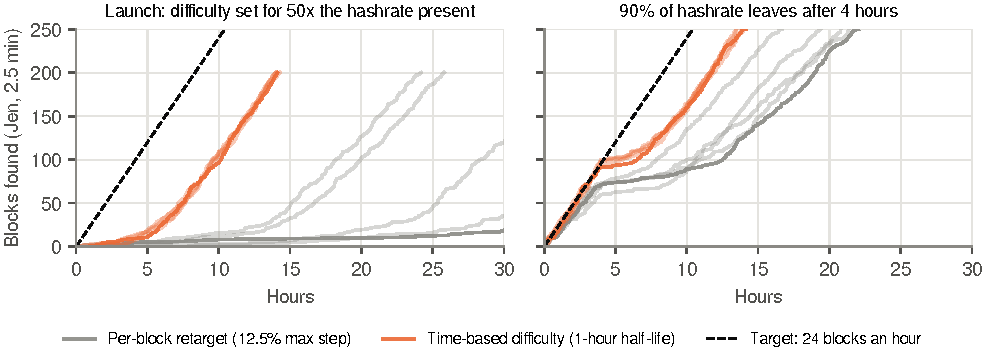
\includegraphics[width=\textwidth]{figs/launch.pdf}
\caption{Launch and hashrate-drop simulation for Jen (five runs per rule, Poisson block discovery; simulated for this paper, Appendix~\ref{app:sims}). Grey: retarget only when a block arrives, at most 12.5\% per block. Orange: time-based difficulty with a one-hour half-life.}
\label{fig:launch}
\end{figure}

\paragraph{Throughput.} A Jen block carries 24 winning blows. With up to 16 payments per blow that is 384 payments per 150-second block, about 2.6 payments per second. Leaves are not tied to blows once minters are credentialed, so the real ceiling is the 1,024-leaf verification limit: up to 16,384 payments a block, about 110 per second. With one stamp per block (benchmarked in Section~\ref{sec:stamp}) the limit becomes the 2\,MB data ceiling at about 16 bytes a payment: about 125,000 payments a block, 830 per second on Jen and about 1,700 per second across the three chains (Figure~\ref{fig:throughput}). Payments beyond that move to channels.
